\chapter{形状微分}
\section{形状微分の公式}

\begin{figure}[ht]
	\begin{center}
		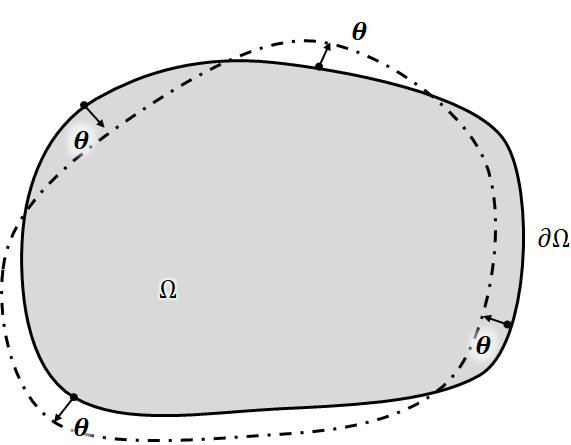
\includegraphics[height=5cm]{./figures/SDFormula.png}
		\caption{Deformation in $\bm{\theta}$ direction}
		\label{fig:SDFormula}
	\end{center}
\end{figure}

形状微分には以下のような公式が存在する.

汎関数$J$が積分領域$\Omega$に依存しない密度関数$f$の領域積分によって,次式のように表されるとする.
\begin{align}
	J=\int_{\Omega}f d\Omega
	\label{eq:functinal_d}
\end{align}
この時,$J$の形状微分は次式で得られる.
\begin{align}
	DJ\cdot\theta=\int_{\Gamma}(\theta_{i}n_{i})f d\Omega
	\label{eq:drivative_d}
\end{align}
ただし,$\bm{n}$は$\Gamma$上の外向きの単位法線ベクトルを表す.

次に,汎関数$J$が密度関数$f$の境界積分によって,次式のように表される場合を考える.
\begin{align}
	J=\int_{\Gamma}f d\Gamma
	\label{eq:functinal_b}
\end{align}
この時,$J$の形状微分は次式で得られる.
\begin{align}
	DJ\cdot\theta=\int_{\Gamma}(\theta_{i}n_{i})\Bigr(\frac{\partial f}{\partial x_{j}}n_{j}+Hf\Bigl) d\Omega
	\label{eq:drivative_b}
\end{align}
ただし,$H\equiv div\bm{n}$は$\Gamma$の平均曲率を表す.

公式\eqref{eq:drivative_d},\eqref{eq:drivative_b}はいずれも密度関数$f$が積分領域に依存しないことが条件であることに注意が必要である.

\section{ラグラジアンの定式化}

\begin{figure}[ht]
	\begin{center}
		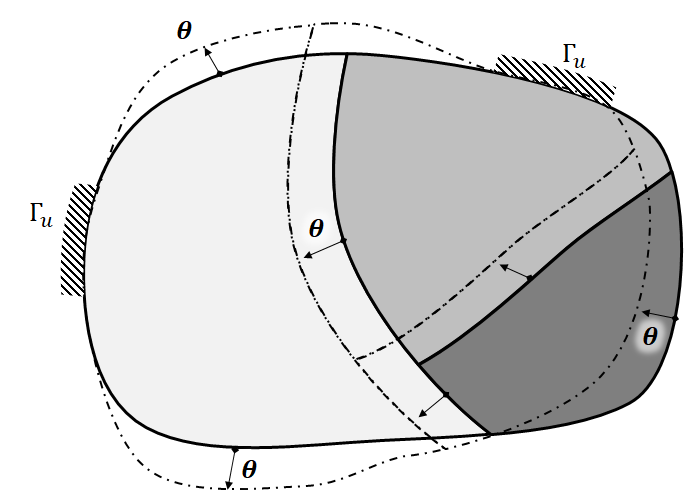
\includegraphics[height=5cm]{./figures/SD.png}
		\caption{Shape derivative}
		\label{fig:SD}
	\end{center}
\end{figure}

ラグラジアンを以下のように定式化する.
\begin{align}
	\mathscr{L}(\Omega_{p\{1\leq p\leq n\}};\bm{U},X,\bm{V},Y)=
	&X+\sum_{p=1}^{n}\int_{\Omega_p}\Bigr( V_{i,j}C_{ijkl}^{p}U_{k,l}-X\rho^{p}V_{i}U_{i}\Bigl) d\Omega
	\nonumber
	\\
	&-\sum_{p=1}^{n-1}\sum_{p=q}^{n}\int_{\Gamma_{pq}}\frac{1}{2}\Bigr(C_{ijkl}^{p}U_{k,l}^{p}n_{j}^{p}-C_{ijkl}^{q}U_{k,l}^{q}n_{j}^{q}\Bigl)(V_{i}^{p}-V_{i}^{q}) d\Gamma
	\nonumber
	\\
	&-\sum_{p=1}^{n-1}\sum_{p=q}^{n}\int_{\Gamma_{pq}}\frac{1}{2}\Bigr(V_{i,j}^{p}C_{ijkl}^{p}n_{l}^{p}-V_{i,j}^{q}C_{ijkl}^{q}n_{l}^{q}\Bigl)(U_{k}^{p}-U_{k}^{q})d\Gamma
	\nonumber
	\\
	&-\sum_{p=1}^{n}\int_{\Gamma_{pu}}\Bigr(C_{ijkl}^{p}U_{k,l}^{p}n_{j}^{p}\Bigl)(V_{i}^{p}) d\Gamma
	\nonumber
	\\
	&-\sum_{p=1}^{n}\int_{\Gamma_{pu}}\Bigr(V_{i,j}^{p}C_{ijkl}^{p}n_{l}^{p}\Bigl)(U_{k}^{p}) d\Gamma
	\nonumber
	\\
	&+Y\Bigr\{1- \sum_{p=1}^{n}\int_{\Omega_{p}}(\rho^{p}U_{i}U_{i}) d\Omega \Bigl\}
	\label{eq:lagrange}
\end{align}
$\bm{U},X$はそれぞれ状態変数$\bm{u},\lambda$に対応する変数,$\bm{V},Y$はラグランジュ乗数である.
ここで,$\bm{u}$や$\lambda$が領域$\Omega_p$に依存する関数であるのに対し,$\bm{U},X,\bm{V},Y$は$\Omega_p$に依存しない関数であることに注意が必要である.

ラグラジアン\eqref{eq:lagrange}に対し,$\bm{V}$に関して部分積分を行うと
\begin{align}
	\mathscr{L}(\Omega_{p\{1\leq p\leq n\}};\bm{U},X,\bm{V},Y)=&X-\sum_{p=1}^{n}\int_{\Omega_p}\Bigr(C_{ijkl}^{p}U_{k,lj}+X\rho^{p}U_{i}\Bigl)V_{i} d\Omega
	\nonumber
	\\
	&+\sum_{p=1}^{n-1}\sum_{p=q}^{n}\int_{\Gamma_{pq}}\frac{1}{2}\Bigr(C_{ijkl}^{p}U_{k,l}^{p}n_{j}^{p}+C_{ijkl}^{q}U_{k,l}^{q}n_{j}^{q}\Bigl)(V_{i}^{p}-V_{i}^{q}) d\Gamma
	\nonumber
	\\
	&-\sum_{p=1}^{n-1}\sum_{p=q}^{n}\int_{\Gamma_{pq}}\frac{1}{2}\Bigr(V_{i,j}^{p}C_{ijkl}^{p}n_{l}^{p}-V_{i,j}^{q}C_{ijkl}^{q}n_{l}^{q}\Bigl)(U_{k}^{p}-U_{k}^{q})d\Gamma
	\nonumber
	\\
	&+\sum_{p=1}^{n}\int_{\Gamma_{pN}}\Bigr(C_{ijkl}^{p}U_{k,l}^{p}n_{j}^{p}\Bigl)(V_{i}^{p}) d\Gamma
	\nonumber
	\\
	&-\sum_{p=1}^{n}\int_{\Gamma_{pu}}\Bigr(V_{i,j}^{p}C_{ijkl}^{p}n_{l}^{p}\Bigl)(U_{k}^{p}) d\Gamma
	\nonumber
	\\
	&+Y\Bigr\{1- \sum_{p=1}^{n}\int_{\Omega_{p}}(\rho^{p}U_{i}U_{i}) d\Omega \Bigl\}
	\nonumber
	\\
	\label{eq:lagrange_vint}
\end{align}
状態方程式\eqref{eq:govmain}~\eqref{eq:govnorm}より,$\bm{U}=\bm{u}(\Omega_{p\{1\leq p\leq n\}})$,
$X=\lambda(\Omega_{p\{1\leq p\leq n\}})$とすれば,任意の$\bm{V},Y$に対して次式が成立することがわかる.
\begin{align}
	\mathscr{L}(\Omega_{p\{1\leq p\leq n\}};\bm{u},\lambda,\bm{U},Y)=\lambda(\Omega_{p\{1\leq p\leq n\}})
	\label{eq:Lagrange_lambda}
\end{align}

\section{ラグラジアンの停留条件}

式\eqref{eq:Lagrange_lambda}より,$\lambda(\Omega_{p\{1\leq p\leq n\}})$の形状微分は次式のように表される.
\begin{align}
	D\lambda(\Omega_{p\{1\leq p\leq n\}})\cdot\bm{\theta}
	=&D\mathscr{L}(\Omega_{p\{1\leq p\leq n\}};\bm{u},\lambda,\bm{V},Y)\cdot\bm{\theta}
	\nonumber
	\\
	&+\Bigr\langle \frac{\partial \mathscr{L}}{\partial \bm{V}}(\Omega_{p\{1\leq p\leq n\}};\bm{u},\lambda,\bm{V},Y),
	\delta\bm{u} \Bigl\rangle
	\nonumber
	\\
	&+\frac{\partial \mathscr{L}}{\partial X}(\Omega_{p\{1\leq p\leq n\}};\bm{u},\lambda,\bm{V},Y)\cdot
	\delta\lambda
	\label{eq:shape_lagrange}
\end{align}
ここで,$\delta\bm{u}$および$\delta\lambda$はそれぞれ状態場$\bm{u}$および$\lambda$の変分である.
$\bm{u}$および$\lambda$が状態方程式を介して領域$\Omega_{p}$に依存しているため,連鎖率によって上式の右辺第2項および第3項が生じている.
しかし,$\delta\bm{u}$および$\delta\lambda$は導出することが困難であるため,
それらの計算を回避するためにラグラジアンの停留条件を考える.
\begin{align}
	\left.\bigr\langle \frac{\partial \mathscr{L}}{\partial \bm{U}},\delta \bm{U} \bigl\rangle\right|_{opt}=0
	\label{eq:optc_u}
	\\
	\left.\frac{\partial\mathscr{L}}{\partial X}\right|_{opt}=0
	\label{eq:optc_x}
	\\
	\left.\bigr\langle \frac{\partial \mathscr{L}}{\partial \bm{V}},\delta \bm{V} \bigl\rangle\right|_{opt}=0
	\label{eq:optc_v}
	\\
	\left.\frac{\partial\mathscr{L}}{\partial Y}\right|_{opt}=0
	\label{eq:optc_y}
\end{align}
まず,式\eqref{eq:optc_v},\eqref{eq:optc_y}に関しては,式\eqref{eq:lagrange_vint}より次式のようになる.
\begin{align}
	0=&\left.\bigr\langle \frac{\partial \mathscr{L}}{\partial \bm{V}},\delta \bm{V} \bigl\rangle\right|_{opt}
	\nonumber
	\\
	=&\sum_{p=1}^{n}\int_{\Omega_p}\Bigr(C_{ijkl}^{p}U_{k,lj}+X\rho^{p}U_{i}\Bigl)\delta V_{i} d\Omega
	\nonumber
	\\
	&+\sum_{p=1}^{n-1}\sum_{p=q}^{n}\int_{\Gamma_{pq}}\frac{1}{2}\Bigr(C_{ijkl}^{p}U_{k,l}^{p}n_{j}^{p}+C_{ijkl}^{q}U_{k,l}^{q}n_{j}^{q}\Bigl)(\delta V_{i}^{p}-\delta V_{i}^{q}) d\Gamma
	\nonumber
	\\
	&-\sum_{p=1}^{n-1}\sum_{p=q}^{n}\int_{\Gamma_{pq}}\frac{1}{2}\Bigr(\delta V_{i,j}^{p}C_{ijkl}^{p}n_{l}^{p}-\delta V_{i,j}^{q}C_{ijkl}^{q}n_{l}^{q}\Bigl)(U_{k}^{p}-U_{k}^{q})d\Gamma
	\nonumber
	\\
	&+\sum_{p=1}^{n}\int_{\Gamma_{pN}}\Bigr(U_{i,j}^{p}C_{ijkl}^{p}n_{l}^{p}\Bigl)(\delta V_{i}^{p}) d\Gamma
	\nonumber
	\\
	&-\sum_{p=1}^{n}\int_{\Gamma_{pu}}\Bigr(\delta V_{i,j}^{p}C_{ijkl}^{p}n_{l}^{p}\Bigl)(U_{k}^{p}) d\Gamma
	\label{eq:lagrange_vderivative}
\end{align}
\begin{align}
	0=\left.\frac{\partial \mathscr{L}}{\partial Y}\right|_{opt}=1- \sum_{p=1}^{n}\int_{\Omega_{p}}(\rho^{p}U_{i}U_{i}) d\Omega
	\label{eq:lagrange_yderivative}
\end{align}
上式と状態方程式\eqref{eq:govmain}~\eqref{eq:govnorm}との比較から,$\bm{U}=\bm{u}(\Omega_{p\{1\leq p\leq n\}})$,$X=\lambda(\Omega_{p\{1\leq p\leq n\}})$の時,
任意の$\delta \bm{V}$に対して停留条件\eqref{eq:optc_v},\eqref{eq:optc_y}が成立することがわかる.

$\bm{V}=\bm{v}(\Omega_{p\{1\leq p\leq n\}}),Y=\eta(\Omega_{p\{1\leq p\leq n\}})$が$\bm{U},X$に関する停留条件\eqref{eq:optc_u},\eqref{eq:optc_x}
を満たすとすると,$\lambda$の形状微分は以下のように表される.
\begin{align}
	D\lambda(\Omega_{p\{1\leq p\leq n\}})\cdot\bm{\theta}
	=&D\mathscr{L}(\Omega_{p\{1\leq p\leq n\}};\bm{u},\lambda,\bm{v},\eta)\cdot\bm{\theta}
	\nonumber
	\\
	&+\Bigr\langle \frac{\partial \mathscr{L}}{\partial \bm{U}}(\Omega_{p\{1\leq p\leq n\}};\bm{u},\lambda,\bm{v},\eta),
	\delta\bm{u} \Bigl\rangle
	\nonumber
	\\
	&+\frac{\partial \mathscr{L}}{\partial X}(\Omega_{p\{1\leq p\leq n\}};\bm{p},\lambda,\bm{v},\eta)\cdot
	\delta\lambda
	\nonumber
	\\
	&+\Bigr\langle \frac{\partial \mathscr{L}}{\partial \bm{V}}(\Omega_{p\{1\leq p\leq n\}};\bm{u},\lambda,\bm{v},\eta),
	\delta\bm{v} \Bigl\rangle
	\nonumber
	\\
	&+\frac{\partial \mathscr{L}}{\partial Y}(\Omega_{p\{1\leq p\leq n\}};\bm{p},\lambda,\bm{v},\eta)\cdot
	\delta\eta
	\nonumber
	\\
	=&D\mathscr{L}(\Omega_{p\{1\leq p\leq n\}};\bm{u},\lambda,\bm{v},\eta)\cdot\bm{\theta}
	\label{eq:shape_lambda_uv}
\end{align}
ここで,上式の中辺第2項から第5項が停留条件\eqref{eq:optc_u}~\eqref{eq:optc_y}より,
任意の$\delta\bm{u},\delta\lambda,\delta\bm{v},\delta\eta$に対して0になることを用いた.
式\eqref{eq:shape_lambda_uv}より,ラグラジアンの形状微分の式に$\bm{U}=\bm{u},X=\lambda,\bm{V}=\bm{v},Y=\eta$
を代入することで,固有値$\lambda$の形状微分が得られることが分かる.

\section{随伴方程式}
続いて,$\bm{U},X$に関する停留条件\eqref{eq:optc_u},\eqref{eq:optc_x}をみたすような,
$\bm{V}=\bm{v}(\Omega_{p\{1\leq p\leq n\}}),Y=\eta(\Omega_{p\{1\leq p\leq n\}})$の条件について考える.

ラグラジアン\eqref{eq:lagrange}に対し,$\bm{U}$に関して部分積分を行うと
\begin{align}
	\mathscr{L}(\Omega_{p\{1\leq p\leq n\}};\bm{U},X,\bm{V},Y)=&X-\sum_{p=1}^{n}\int_{\Omega_p}\Bigr(V_{i,jl}C_{ijkl}^{p}+X\rho^{p}V_{k}\Bigl)U_{k} d\Omega
	\nonumber
	\\
	&-\sum_{p=1}^{n-1}\sum_{p=q}^{n}\int_{\Gamma_{pq}}\frac{1}{2}\Bigr(C_{ijkl}^{p}U_{k,l}^{p}n_{j}^{p}-C_{ijkl}^{q}U_{k,l}^{q}n_{j}^{q}\Bigl)(V_{i}^{p}-V_{i}^{q}) d\Gamma
	\nonumber
	\\
	&+\sum_{p=1}^{n-1}\sum_{p=q}^{n}\int_{\Gamma_{pq}}\frac{1}{2}\Bigr(V_{i,j}^{p}C_{ijkl}^{p}n_{l}^{p}+V_{i,j}^{q}C_{ijkl}^{q}n_{l}^{q}\Bigl)(U_{k}^{p}-U_{k}^{q})d\Gamma
	\nonumber
	\\
	&+\sum_{p=1}^{n}\int_{\Gamma_{pN}}\Bigr(V_{i,j}^{p}C_{ijkl}^{p}n_{l}^{p}\Bigl)(U_{k}^{p}) d\Gamma
	\nonumber
	\\
	&-\sum_{p=1}^{n}\int_{\Gamma_{pu}}\Bigr(C_{ijkl}^{p}U_{k,l}^{p}n_{j}^{p}\Bigl)(V_{i}^{p}) d\Gamma
	\nonumber
	\\
	&+Y\Bigr\{1- \sum_{p=1}^{n}\int_{\Omega_{p}}(\rho^{p}U_{i}U_{i}) d\Omega \Bigl\}
	\nonumber
	\\
	\label{eq:lagrange_uint}
\end{align}
となるため,停留点における$\bm{V}$および$Y$をそれぞれ$\bm{v}$,$\eta$とすると,式\eqref{eq:optc_u},\eqref{eq:optc_x}は以下のようになる.
\begin{align}
	0=&\left.\bigr\langle \frac{\partial \mathscr{L}}{\partial \bm{U}},\delta \bm{U} \bigl\rangle\right|_{opt}
	\nonumber
	\\
	=&\sum_{p=1}^{n}\int_{\Omega_p}\Bigr(v_{k,lj}C_{ijkl}^{p}+\lambda\rho^{p}v_{i}+2\eta\rho^{p}u_{i}\Bigl)\delta U_{i} d\Omega
	\nonumber
	\\
	&-\sum_{p=1}^{n-1}\sum_{p=q}^{n}\int_{\Gamma_{pq}}\frac{1}{2}\Bigr(\delta U_{i,j}^{p}C_{ijkl}^{p}n_{l}^{p}-\delta U_{i,j}^{q}C_{ijkl}^{q}n_{l}^{q}\Bigl)(v_{k}^{p}-v_{k}^{q}) d\Gamma
	\nonumber
	\\
	&+\sum_{p=1}^{n-1}\sum_{p=q}^{n}\int_{\Gamma_{pq}}\frac{1}{2}\Bigr(v_{k,l}^{p}C_{ijkl}^{p}n_{j}^{p}+v_{k,l}^{q}C_{ijkl}^{q}n_{j}^{q}\Bigl)(\delta U_{i}^{p}-\delta U_{i}^{q})d\Gamma
	\nonumber
	\\
	&+\sum_{p=1}^{n}\int_{\Gamma_{pN}}\Bigr(v_{k,l}^{p}C_{ijkl}^{p}n_{j}^{p}\Bigl)\delta U_{i}^{p} d\Gamma
	\nonumber
	\\
	&-\sum_{p=1}^{n}\int_{\Gamma_{pu}}\Bigr(\delta U_{i,j}^{p}C_{ijkl}^{p}n_{l}^{p}\Bigl)v_{k}^{p} d\Gamma
	\label{eq:lagrange_uderivative}
\end{align}
\begin{align}
	0=\left.\frac{\partial\mathscr{L}}{\partial X}\right|_{opt}
	=1-\sum_{p=1}^{n}\int_{\Omega_p}\bigr(\rho^{p}v_{i}u_{i}\bigl) d\Omega
	\label{eq:lagrange_xderivative}
\end{align}
ここで,$C_{ijkl}=C_{klij}$であることを用いて,添え字を$(i,j,k,l)\rightarrow(k,l,i,j)$に変換した.
以上から,$\bm{v}$,$\eta$が以下の随伴方程式を満たすとき,停留条件\eqref{eq:optc_u},\eqref{eq:optc_x}は成立する.
\begin{align}
	&C_{ijkl}^{p}v_{k,lj}+\lambda\rho^{p}v_{i}+2\eta\rho^{p} u_{i}=0&\text{in}\hspace{0.3cm}\Omega_{p}
	\label{eq:adjmain}
	\\
	&v_{i}=0 &\text{on}\hspace{0.3cm}\Gamma_{D}
	\\
	&C_{ijkl}v_{k,l}^{}n_{j}=0 &\text{on}\hspace{0.3cm}\Gamma_{N}
	\\
	&v_{i}^{p}=v_{i}^{q} &\text{on}\hspace{0.3cm}\Gamma_{pq}
	\\
	&C_{ijkl}^{p}v_{k,l}^{p}n_{j}^{p}+C_{ijkl}^{q}v_{k,l}^{q}n_{j}^{q}=0 &\text{on}\hspace{0.3cm}\Gamma_{pq}
	\label{eq:adjbc}
	\\
	&\sum_{p=1}^{n}\int_{\Omega_p}(\rho^{p}v_{i}u_{i}) d\Omega=1
	\label{eq:adjnorm}
\end{align}
次に,$\eta$の値を求める.
まず,強形式の状態方程式\eqref{eq:govmain}に$\bm{v}$をかけ,領域積分することで次式が得られる.
\begin{align}
	\sum_{p=1}^{n}\int_{\Omega_p}\Bigr(v_{i,j}C_{ijkl}^{p}u_{k,l}-\lambda\rho^{p}v_{i}u_{i}\Bigl) d\Omega=0
	\label{eq:gov_p}
\end{align}
強形式の随伴方程式\eqref{eq:adjmain}に$\bm{u}$をかけ,領域積分することで次式が得られる.
\begin{align}
	\sum_{p=1}^{n}\int_{\Omega_p}\Bigr(v_{i,j}C_{ijkl}^{p}u_{k,l}-\lambda\rho^{p}u_{i}^{}v_{i}^{}-2\eta u_{i}^{}u_{i}^{}\Bigl) d\Omega=0
	\label{eq:adj_u}
\end{align}
式\eqref{eq:gov_p}と式\eqref{eq:adj_u}の差を取り,正規化条件\eqref{eq:govnorm}を用いることで以下のように$\eta$が求まる.
\begin{align}
	\eta\sum_{p=1}^{n}\int_{\Omega_p}(\rho^{p}u_{i}^{}u_{i}^{}) d\Omega=\eta=0
	\label{eq:eta_0}
\end{align}
ゆえに,随伴場の偏微分方程式\eqref{eq:adjmain}~\eqref{eq:adjbc}は状態場の偏微分方程式\eqref{eq:govmain}~\eqref{eq:govbc}と等しくなり,
随伴場$\bm{v}$は次式のように状態場$\bm{u}$の定数倍で与えられる.
\begin{align}
	\bm{v}=K\bm{u}
	\label{eq:v_ku}
\end{align}
さらに,状態場と随伴場の正規化条件\eqref{eq:govnorm},\eqref{eq:adjnorm}より,次式のようにKの値が求まる.
\begin{align}
	1&=\sum_{p=1}^{n}\int_{\Omega_p}\Bigr(\rho^{p}u_{i}v_{i}\Bigl) d\Omega
	\nonumber
	\\
	&=K\sum_{p=1}^{n}\int_{\Omega_p}\Bigr(\rho^{p}u_{i}u_{i}\Bigl) d\Omega
	\nonumber
	\\
	&=K
	\label{eq:k}
\end{align}
ゆえに,$\bm{u}$と$\bm{v}$は等しい.
\begin{align}
	\bm{v}=\bm{u}
	\label{eq:v_u}
\end{align}

\section{形状微分の公式の適用}

式\eqref{eq:shape_lambda_uv}に式\eqref{eq:eta_0},\eqref{eq:v_u}を代入することで,
固有値$\lambda$の形状微分は次式のように表される.
\begin{align}
	D\lambda\cdot\bm{\theta}
	=&D\mathscr{L}(\Omega_{p\{1\leq p\leq n\}};\bm{u},\lambda,\bm{u},0)\cdot\bm{\theta}
	\label{eq:shape_lambda_u}
\end{align}

形状微分の公式\eqref{eq:drivative_d},\eqref{eq:drivative_b}を式\eqref{eq:shape_lambda_u}のラグラジアンの形状微分に適用し,
$\Gamma_{u}$上で$\bm{\theta}=\bm{0}$を仮定すると次式が得られる.
\begin{align}
	&\hspace{0.5cm}D\lambda\cdot\bm{\theta}
	\nonumber
	\\
	&=D\mathscr{L}(\Omega_{p\{1\leq p\leq n\}};\bm{u},\lambda,\bm{u},0)\cdot\bm{\theta}
	\nonumber
	\\
	&=\sum_{p=1}^{n}\int_{\Gamma_p}(\theta_{m}n_{m}^{p})\Bigr(u_{i,j}C_{ijkl}^{p}u_{k,l}-\lambda\rho^{p}u_{i}u_{i}\Bigl) d\Omega
	\nonumber
	\\
	&-\sum_{p=1}^{n-1}\sum_{p=q}^{n}\int_{\Gamma_{pq}}(\theta_{m}n_{m}^{p})
	\Bigr(\frac{\partial}{\partial x_\gamma }n_\gamma^{p} +H^{p}\Bigl)
	\Bigr(C_{ijkl}^{p}u_{k,l}^{p}n_{j}^{p}-C_{ijkl}^{q}u_{k,l}^{q}n_{j}^{q}\Bigl)
	(u_{i}^{p}-u_{i}^{q}) d\Gamma
	\label{eq:shape_lambda}
\end{align}
境界条件から$\partial \Omega_{pq}$上で$\bm{u}^{p}=\bm{u}^{q}$であることに注意すると,
固有値$\lambda$の形状微分は次式のように導出される.
\begin{align}
	\hspace{0.5cm}D\lambda\cdot\bm{\theta}
	=&\sum_{p=1}^{n}\int_{\Gamma_p}(\theta_{m}n_{m}^{p})\Bigr(u_{i,j}C_{ijkl}^{p}u_{k,l}-\lambda\rho^{p}u_{i}u_{i}\Bigl) d\Omega
	\nonumber
	\\
	&-\sum_{p=1}^{n-1}\sum_{p=q}^{n}\int_{\Gamma_{pq}}(\theta_{m}n_{m}^{p})
	\Bigr(C_{ijkl}^{p}u_{k,l}^{p}n_{j}^{p}-C_{ijkl}^{q}u_{k,l}^{q}n_{j}^{q}\Bigl)
	(u_{i,\gamma}^{p}n_\gamma^{p}-u_{i,\gamma}^{q}n_\gamma^{p}) d\Gamma
	\label{eq:shape_lambda}
\end{align}


